 % Local variables:
 % TeX-open-quote: "\"`"
 % TeX-close-quote: "\"'"
 % End:



\part{Forschungssynthese als sozialwissenschaftliche Methode}\label{part:forsch-als-sozi}
\frame{\partpage}

\frame{\frametitle{Forschungssynthese als sozialwissenschaftliche Methode}
  \tableofcontents[part=3, hideallsubsections]}


\section{Der sozialwissenschaftliche Forschungsprozess}

\begin{frame}\frametitle{Relevante Dimensionen des Forschungsdesigns}
  \begin{itemize*}
  \item Wahl der Untersuchungseinheiten (bspw. Individuen vs. Kollektive)
  \item \textbf{Untersuchungsarten}
    \begin{itemize}
    \item Primäranalyse
    \item Sekundäranalyse
    \item Meta-Analyse
    \end{itemize}
  \item Zeitdimension (Querschnitt vs. Längsschnitt)
  \end{itemize*}
\end{frame}


\begin{frame}
  \frametitle{Untersuchungsarten}
  \begin{itemize*}
  \item<+-> \textbf{Primäranalyse}: Erstmalige Nutzung und Auswertung \emph{eines} Datensatzes.
  \item<+-> \textbf{Sekundäranalyse}: Erneute Nutzung \emph{eines} Datensatzes unter geänderten Bedingungen der
    Forschungsmethodik und\,/\,oder des theoretischen Bezugssystems.
  \item<+-> \textbf{Meta-Analyse}: Nutzung und Auswertung \emph{mehrerer} Datensätze\,/\,Studien mit gemeinsamer
    Fragestellung (womit noch \emph{nichts} über die Analyseeinheit gesagt wird!).
  \end{itemize*}
\end{frame}


\begin{frame}
  \frametitle{Elemente einer quantitativen Forschungssynthese}
  \begin{small}
    \begin{columns}[t]
    %%
      \begin{column}{0.35\linewidth}
        Diekmann (1997)
        \begin{enumerate}
        \item Formulierung und Präzisierung des Forschungsproblems
        \item Planung und Vorbereitung der Erhebung
        \item Datenerhebung
        \item Daten\-auswertung
        \item Berichterstattung
        \end{enumerate}
      \end{column}
      %%
      \begin{column}{0.3\linewidth}
        Cooper (1982)
        \begin{enumerate}
        \item Problem Formulation
        \item Data Collection
        \item Data Evaluation
        \item Analysis and Interpretation
        \item Public Presentation
        \end{enumerate}
      \end{column}
      %%
      \begin{column}{0.34\linewidth}
        Wagner\,/\,Weiß (2003)
        \begin{enumerate}
        \item Problem\,/\,\\Forschungsfrage
        \item Literatur-\- oder Datensatz\-recherche\- (allg. Datenerhebung)
        \item Dateneingabe
        \item Datenanalyse (Meta-Analyse)
        \item Ergebnis\-präsentation
        \end{enumerate}
      \end{column}
      %%
    \end{columns}
  \end{small}
\end{frame}



\section{Forschungsfrage}

\begin{frame}
  \frametitle{Bedeutung der Forschungsfrage}
  %%
  \begin{itemize}[<+->]
  \item Die Forschungsfrage \emph{muss} die interessierenden Merkmale und Zusammenhänge präzise beschreiben, um (später)
    relevante und irrelevante Studien/Publikationen voneinander unterscheiden zu können.
  \item Aus der Forschungsfrage lassen/sollten sich Kriterien für die Wahl relevanter bzw. irrelevanter Studien ableiten.
  \end{itemize}
\end{frame}


\begin{frame}
  \frametitle{Kriterien für eine gelungene Forschungsfrage}
  \begin{itemize}[<+->]
  \item Interessierende Variablen/Merkmale wurden klar definiert ("`Konzeptspezifikation"').
  \item Relevantes Forschungsdesign spezifizieren.
  \item Die Forschungsfrage in einen historischen, geographischen, theoretischen, methodologischen Kontext einbetten.
  \end{itemize}
\end{frame}


\begin{frame}[plain]
  \frametitle{Beispiel für Fragestellung (Wagner/Weiß 2006)}
  %%
  \begin{small}
    "`The aim of this paper is to summarize \alert{European} research on various \alert{divorce risks}. More precisely,
    we will examine how much divorce risks vary between European countries and whether such variations can be explained by
    country-specific macro-level factors. Are there any meaningful differences in the divorce risks between European
    countries?"'
  \end{small}
\end{frame}


\begin{frame}
  \frametitle{Beispiel für Fragestellung (Weiß 2008)}
  %%
  \begin{enumerate}[<+->]
  \item Wie viele Jugendliche schwänzen insgesamt die Schule?
  \item Wie hoch ist das Schulschwänzrisiko bei Jugendlichen mit Migrationshintergrund?
  \item Unterscheidet sich das Schulschwänzrisiko bei Jugendlichen mit Migrationshintergrund an Hauptschulen von den
    übrigen Schulformen?
  \end{enumerate}
\end{frame}


    \begin{frame}
      \frametitle{Beispiel für Fragestellung  (Wilson et al. 2008)}
      %%
      "`Objectives: To synthesize the extant empirical evidence on the effects of
      boot-camps and boot camp like programs on the criminal behavior (e.g., postrelease arrest, conviction, or
      reinstitutionalization) of convicted adult and juvenile offenders."'
    \end{frame}




\section{Datenerhebung: Literatur- und Studienrecherche}

\begin{frame}
  \frametitle{Ziel der (Literatur-)Recherche}
  %%
  Die Literaturrecherche entspricht der Phase der Datenerhebung im Rahmen einer Primäruntersuchung.
  \begin{itemize}[<+->]
  \item Erfassung eines möglichst großen Teiles der vorhandenen Literatur (Vollerhebung).
  \item Vermeidung von Verzerrungen:
    \begin{quotation}
      "`The point is not to track down every paper that is somehow related to
      the topic. (\ldots) The point is to avoid missing a useful paper that lies
      outside one's regular purview"' \citep[44]{white_scientific_1994}.
    \end{quotation}
  \item Systematische und transparente Suche.
  \end{itemize}
\end{frame}



\begin{frame}
  \frametitle{Spezifizierung des Untersuchungsgegenstandes der Forschungssynthese}
  \begin{itemize}[<+->]
  \item Abgrenzung zu anderen, verwandten Themen
  \item Definition der Grundgesamtheit
  \item Wichtige Untersuchungsvariablen
  \item Methodische Anforderungen
  \item Kulturelle und sprachliche Grenzziehungen
  \item \ldots
  \end{itemize}
\end{frame}



\subsection{Recherchestrategien}


\begin{frame}[plain]\frametitle{Genauigkeit und Vollständigkeit}
  \begin{center}
    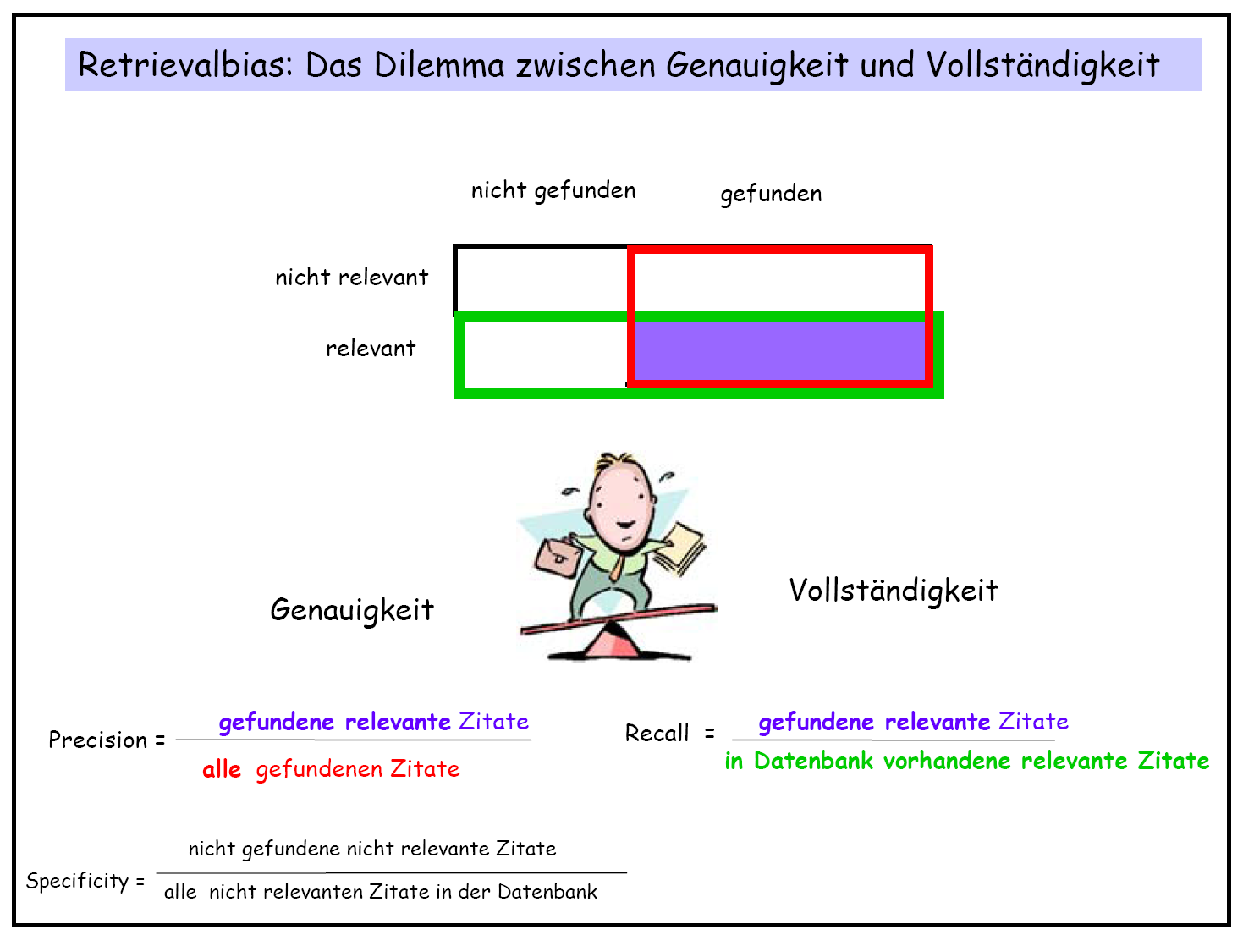
\includegraphics[scale=0.4]{figRecallPrecision}
  \end{center}
  \footnotesize{(Quelle: Motschall 2004: Medline-Suche mit PubMed,
    \url{http://www.agmb.de/04_mannheim/motschall.pdf})}
\end{frame}


\begin{frame}
  \frametitle{Ein unlösbares Problem}
  %%
  \begin{enumerate}[<+->]
  \item \emph{Recall} (Vollständigkeit): Anteil an gefundener relevanter
    Literatur im Verhältnis zur Gesamtzahl (hypothetische Größe) an
    \emph{relevanter} Literatur.
  \item \emph{Präzision} (Präzision, Genauigkeit): Anteil an gefundener
    relevanter Literatur im Verhältnis zur Anzahl \emph{insgesamt gefundener}
    (relevanter und nichtrelevanter) Literatur.
  \item Beide Maße stehen in einer inversen Beziehung und können nicht
    gleichzeitig optimiert werden:
    \begin{itemize}
    \item Je unspezifischer die Suche, desto höher der Recall und desto höher
      der Anteil an irrelevanten Publikationen $\Rightarrow$ hoher Arbeitsaufwand.
    \item Je spezifischer die Suche, desto höher die Precision und desto höher
      die Wahrscheinlichkeit, relevante Untersuchungen zu übersehen
      $\Rightarrow$ Repräsentativität der Stichprobe gefährdet.
    \end{itemize}
  \end{enumerate}
\end{frame}




\begin{frame}
  \frametitle{Suche in Literaturverweisen  ("`footnote chasing"')}
  %%
  \begin{block}{Vorgehen}
    \begin{itemize}[<+->]
    \item Reviews
    \item thematisch verwandte Artikel, Bücher oder Zeitschriften
    \item Bibliographien
    \end{itemize}
  \end{block}
  \pause
  \begin{block}{Beurteilung}
    \begin{itemize}[<+->]
    \item[$+$] guter Einstieg in die Suche
    \item[$+$] meist relativ hohe Präzision
    \item[$-$] selektive, persönliche Auswahl (eigene Untersuchungen / Literaturverweise) $\rightarrow$ Verzerrungen
    \item[$-$] Aktualität der Literatur hängt von Referenzquelle ab. 
    \end{itemize}
  \end{block}
\end{frame}


\begin{frame}
  \frametitle{Suche in (Fach-)Datenbanken: Vorgehen}
  %%
  \begin{itemize}[<+->]
  \item z.B. Wiso 3, SOLIS/FORIS, Sociological Abstracts, SocioFile etc.
  \item  Fachdatenbanken umfassen:
    \begin{itemize}
    \item  meist nur publizierte Artikel
    \item ab einem bestimmten Jahr
    \item innerhalb bestimmter geographischer Grenzen $\rightarrow$ deswegen: Charakteristika der Datenbanken beachten
    \end{itemize}
  \item Übereinstimmung von Suchabfrage mit den Angaben in der Datenbank notwendig $\rightarrow$ richtige Benutzung
    Boolscher Operationen, vorsichtiger Umgang mit Begriffen
  \end{itemize}
\end{frame}


\begin{frame}
  \frametitle{Suche in (Fach-)Datenbanken: Beurteilung}
  %%
  \begin{itemize}[<+->]
  \item[$+$] Vermeidet Verzerrungen aufgrund persönlicher Auswahl.
  \item[$-$] Relativ niedrige Präzision, sofern die Recall-Rate akzeptabel sein soll.
  \item[$-$] Verzerrungen aufgrund der in die Datenbanken aufgenommenen Artikel.
  \end{itemize}
\end{frame}

\begin{frame}
  \frametitle{Suche in Zitationsdatenbanken}
  %%
  \begin{block}{Vorgehen}
    z.B. Social Science Citation Index
  \end{block}
  \pause
  \begin{block}{Beurteilung}
    \begin{itemize}
    \item[$+$] ermöglicht das Auffinden von Literatur aus unterschiedlichen Fachbereichen
    \item[$+$] umfasst neueste Publikationen
    \item[$+$] relativ hohe Recall-Rate
    \item[$-$] Verzerrungen aufgrund der in die Datenbanken aufgenommenen Artikel
    \end{itemize}
  \end{block}
\end{frame}

\begin{frame}
  \frametitle{Kommunikation mit den peers}
  %%
  \begin{block}{Vorgehen}
    \begin{itemize}
    \item Konferenzen
    \item Anfragen bei Forschern
    \item Anfragen bei staatlichen Einrichtungen
    \end{itemize}
  \end{block}
  \begin{block}{Beurteilung}
    \begin{itemize}
    \item[$+$] ermöglicht Auffinden nicht publizierter Literatur
    \item[$+$] sehr hohe Präzision
    \item[$-$] selektive Auswahl $\rightarrow$ Verzerrungen
    \end{itemize}
  \end{block}
\end{frame}


\begin{frame}\frametitle{Systematische Suche in Bibliotheken und Zeitschriften (Browsing)}

  \begin{block}{Vorgehen}
    \begin{itemize}
    \item Systematisches Durchsuchen von Zeitschriftenjahrgängen (bspw. letzte 10 Jahrgänge von JMF)
    \end{itemize}
  \end{block}
  %%
  \begin{block}{Beurteilung}
    \begin{itemize}
    \item[$-$] meist geringe Präzision, zeitaufwendig
    \item[$+$] thematisch eng gefasste Zeitschriften oder Bibliotheksbereiche können aber die Suche sinnvoll ergänzen
    \end{itemize}
  \end{block}
\end{frame}




\subsection{Bewertung und Auswahlkriterien}


\begin{frame}
  \frametitle{Auswahlkriterien}
  %%%
  \begin{small}
    Die Auswahlkriterien definieren die Grundgesamtheit und betreffen die Generalisierbarkeit der Ergebnisse der
    Forschungssynthese. Relevante Dimensionen sind u.a.:
    \begin{itemize}[<+->]
    \item Forschungsdesign (Längsschnitt/Querschnitt, Experiment/Umfrage/\ldots)
    \item Messung zentraler Konstrukte
    \item Grundgesamtheit der einzelnen Studie (Stichprobenzusammensetzung, Alter, Ost/West, \ldots)
    \item Zeitlicher und geographischer Kontext der Studie (Jahr der Stichprobenerhebung, Publikationsjahr, \ldots)
    \item Qualität der Studien (inkl. ausreichend Daten für Durchführung stat. Analysen)
    \item Publikationstyp (un-/veröffentlichte Literatur, graue Literatur, \ldots)
    \item \ldots
    \end{itemize}
  \end{small}
\end{frame}


\begin{frame}
  \frametitle{Beispiel für Auswahlkriterien (Wagner/Weiß 2006)}
  %%
  \begin{small}
    "`Publications dealing with our research question should meet the following
    criteria to be included in our meta-analysis: on the one hand, we were
    interested in publications in which marital stability is the dependent
    variable.  On the other hand, we limited our search to publications that
    explicitly used European longitudinal data sets. The countries considered
    here are the 18 countries of the European Economic Area (EEA), the candidate
    countries for the European Union, and Switzerland"' (Wagner/Weiß 2006: 487).
  \end{small}
\end{frame}


\begin{frame}
  \frametitle{Beispiel für Auswahlkriterien (Weiß 2008)}
  "`Letztlich orientierte sich die Auswahl geeigneter Datensätze an drei
  Kriterien: (1) Der Datensatz enthält Angaben zur selbst- oder fremdberichteten
  unentschuldigten Schulabwesenheit. Dabei ist gleichgültig, für welchen
  Zeitraum das Schulschwänzen erfasst oder wie präzise die Häufigkeit des
  Phänomens gemessen wurde. (2) Die Datensätze sind für Sekundäranalysen
  verfügbar. (3) Die Stichprobe wurde in Deutschland gezogen, ohne jedoch
  vorauszusetzen, nur Schüler mit deutscher Staatsangehörigkeit zu erfassen"'
  (Weiß 2008).
    \end{frame}


    \begin{frame}
      \frametitle{Beispiel für Auswahlkriterien (Wilson et al. 2008)}
      "`Selection Criteria: The eligibility criteria were (a) that the study
      evaluated a correctional boot camp, shock incarceration, or intensive
      incarceration program; (b) that the study included a comparison group that
      received either probation or incarceration in an alternative facility; (c)
      that the study participants were exclusively under the supervision of the
      criminal or juvenile justice system; and (d) that the study reported a
      post-program measure of criminal behavior, such as arrest or conviction"'
      (Wilson et al. 2008: 2).
    \end{frame}




\subsection{Dokumentation der Recherche und Verwaltung der Quellen}

\begin{frame}
  \frametitle{Verwaltung der Literatur}
  \begin{itemize}[<+->]
  \item Tabellenkalkulation (OO-Calc, MS-Excel).
  \item (Kostenpflichtige) Programmee zur Literaturverwaltung wie Endnote,
    Reference Manager etc.
  \item (Kostenfreie) Programme wie Mendeley, Zotero oder RevMan.
  \end{itemize}
  \emph{Ein} Argument für die Verwendung eines bestimmten Programms ist eine
  offene Schnittstelle auf die bspw. Statistiksoftware zugreifen kann (bieten
  etwa Mendeley oder Zotero).
\end{frame}


\begin{frame}[plain]
  \frametitle{Dokumentation der Literaturrecherche (Weiß 2008)}
  \begin{center}
    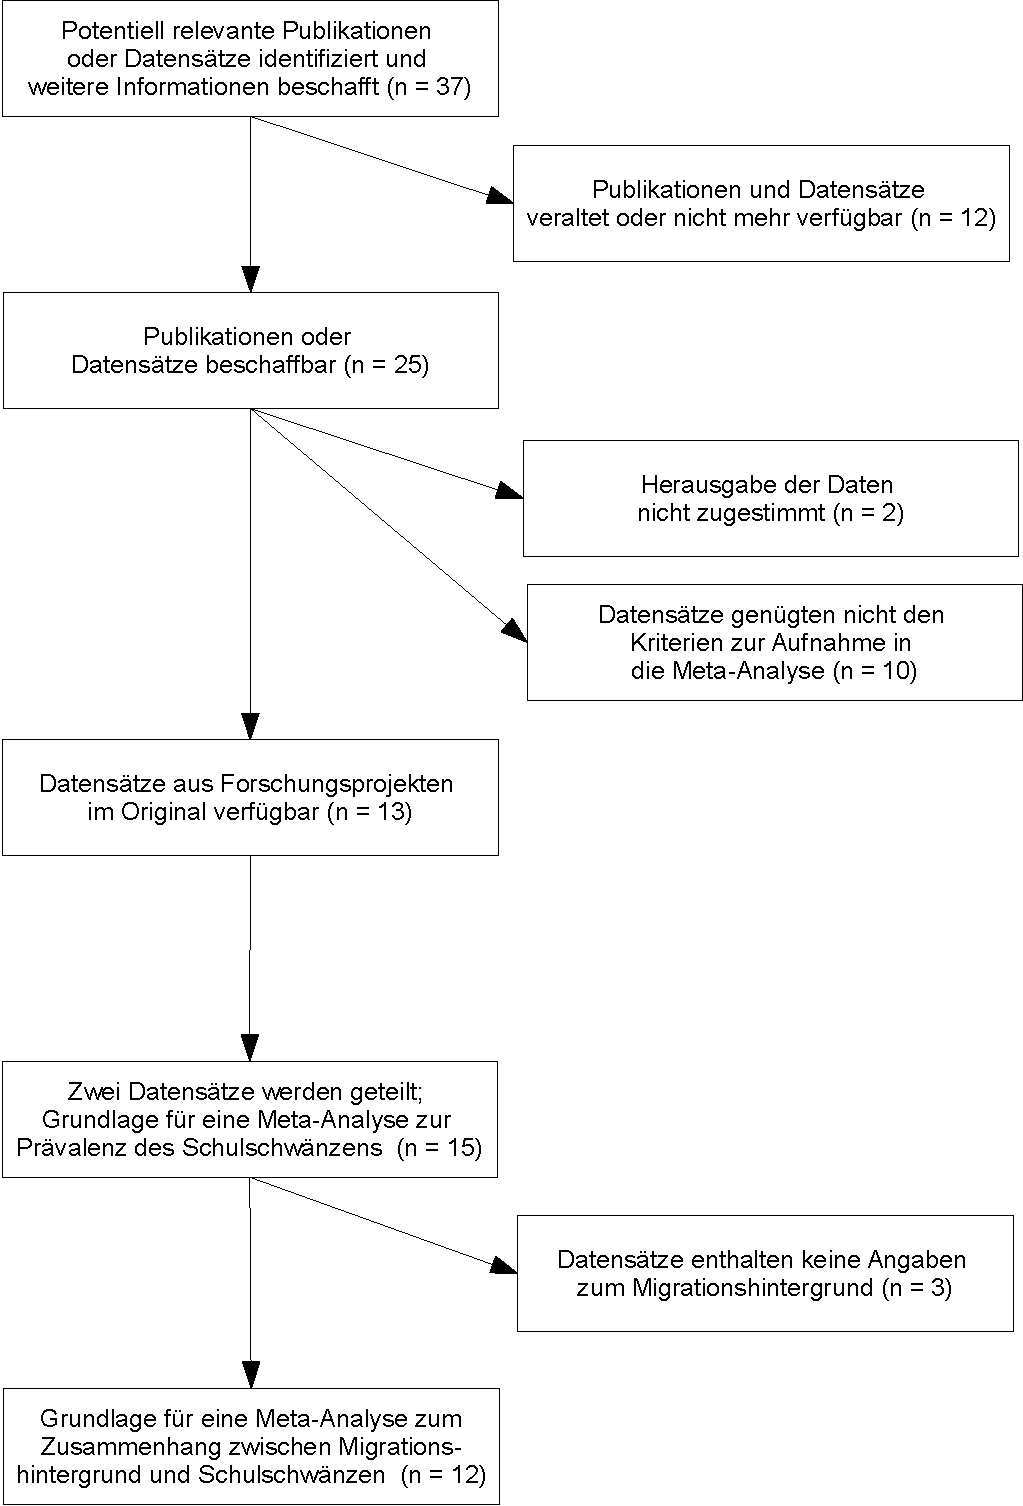
\includegraphics[width = 0.5\textwidth]{figRechercheDatensaetze}
  \end{center}
\end{frame}


\begin{frame}[plain]
  \frametitle{Dokumentation der Literaturrecherche \citep{lorant_socioeconomic_2003}}
  \begin{center}
    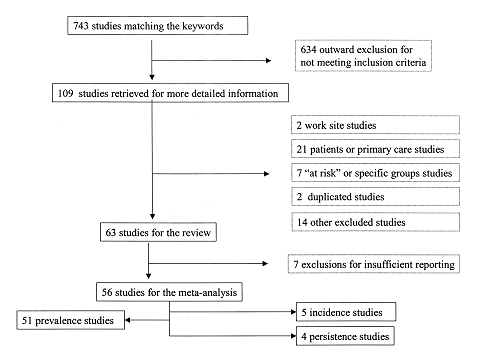
\includegraphics[width=0.85\textwidth]{figDokRechercheLorant}  
  \end{center}
\end{frame}


\subsection{Stichprobenselektivität}

\begin{frame}
  \frametitle{Quellen der Verzerrungen bei der Literatursuche}
  %%
  \begin{itemize}[<+->]
  \item Subjektive Auswahl bei Reviews (ebenfalls eher statistisch signifikante Ergebnisse)
  \item Verzerrung durch Sprachbarrieren
  \item Verzerrung durch einseitige Literaturrecherche
  \item \ldots
  \item $\rightarrow$ Verzerrungen führen tendenziell zu einer Überschätzung der Effektstärken.
  \end{itemize}

  Weitere Informationen zum Thema "`Publication Bias"' finden sich ab Folie \pageref{sec:pubbias}.

\end{frame}

\section{Datenvercodung/-eingabe und Effektstärken}


\begin{frame}
  \frametitle{Übersicht}
  \begin{itemize}[<+->]
  \item Nach der Identifikation relevanter Publikationen müssen die darin enthaltenen Informationen erfasst werden
    (ähnelt einer Inhaltsanalyse).
  \item Festlegen, welche Informationen für die Fragestellung wichtig sind.
  \item Fragebogen (Codierbogen) erstellen.
  \item Insbesondere auf die Vergleichbarkeit der empirischen Befunde achten.
  \end{itemize}
\end{frame}



\begin{frame}
  \frametitle{Datenerhebung und -vercodung}
  \begin{itemize}[<+->]
  \item Welche Informationen aus den Studien besitzen Relevanz (Synthese\,/\,Heterogenität)?
    \begin{itemize}
    \item Publikationsbefunde (Statistiken, Effektstärken, \ldots)
    \item Publikationsmerkmale (Publikationstyp, Publikationsjahr, \ldots)
    \item Studien-/Stichprobenmerkmale (Erhebungsjahr, Organisation, Stichprobendesign, \ldots)
    \item Methode und Qualität (Statistische Verfahren, bestimmte Qualitätskriterien, \ldots)
    \end{itemize}
  \item Konstruktion eines \glq Fragebogens\grq\ (Codierbogen).
  \item Problem: Auswahl überflüssiger oder Auslassen bedeutsamer Variablen.
  \end{itemize}
\end{frame}


% \begin{frame}
%   \frametitle{Studienmerkmale XXX}

%   \begin{itemize}
%   \item Stichprobenquelle
%   \item Stichprobenmerkmale (demographische Angaben: sozioökonomische  Herkunft, Alter, Geschlecht etc.;
%     Personenmerkmale: kognitive Fähigkeiten, Charaktereigenschaften)
%   \item unabhängige Variablen
% 	allgemeine Beschreibung (kategorial oder metrisch etc.)
% 	Ausprägungen
% Methode
% 	Studiendesign

% Quellen der Meta-Analyse
% 	Art der Veröffentlichung (Zeitschrift, Buch, Dissertation etc.)
% 	Publikationsjahr
% 	Sprache in der veröffentlicht wurde
% 	finanzielle Unterstützung der Studie und durch wen
% 	Eigenschaften des Forschers (Geschlecht, Zugehörigkeit zu Institut XY etc.)
%   \end{itemize}
% \end{frame}


\begin{frame}
  \frametitle{Beispiel für Codierbogen (Auszug)}
  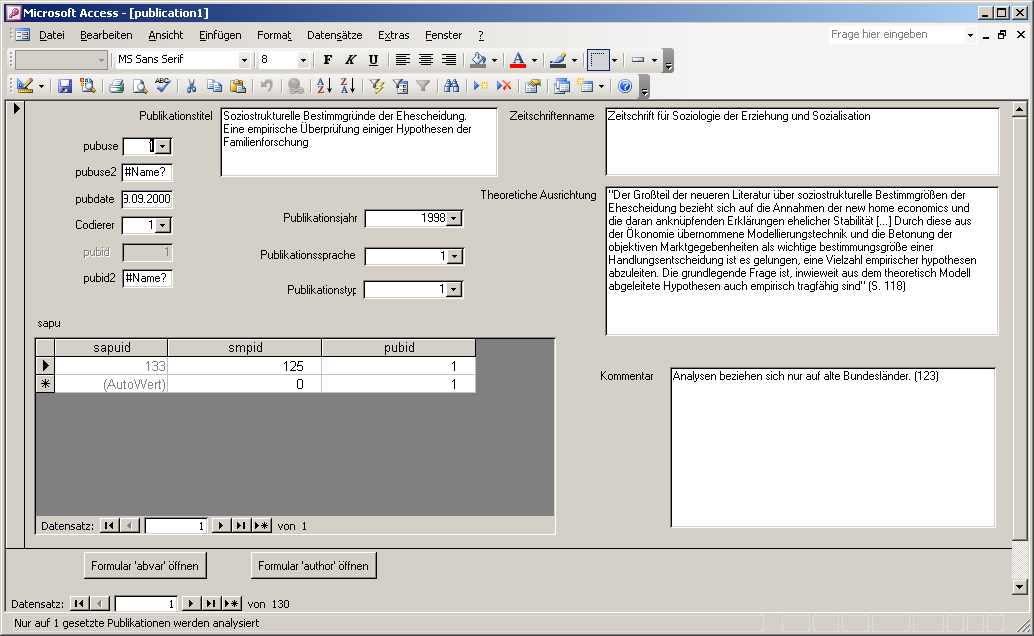
\includegraphics[scale = 0.3]{figCodierbogenScheidung}
\end{frame}


\begin{frame}
  \frametitle{Beispiel für Codierbogen  (Auszug)}
  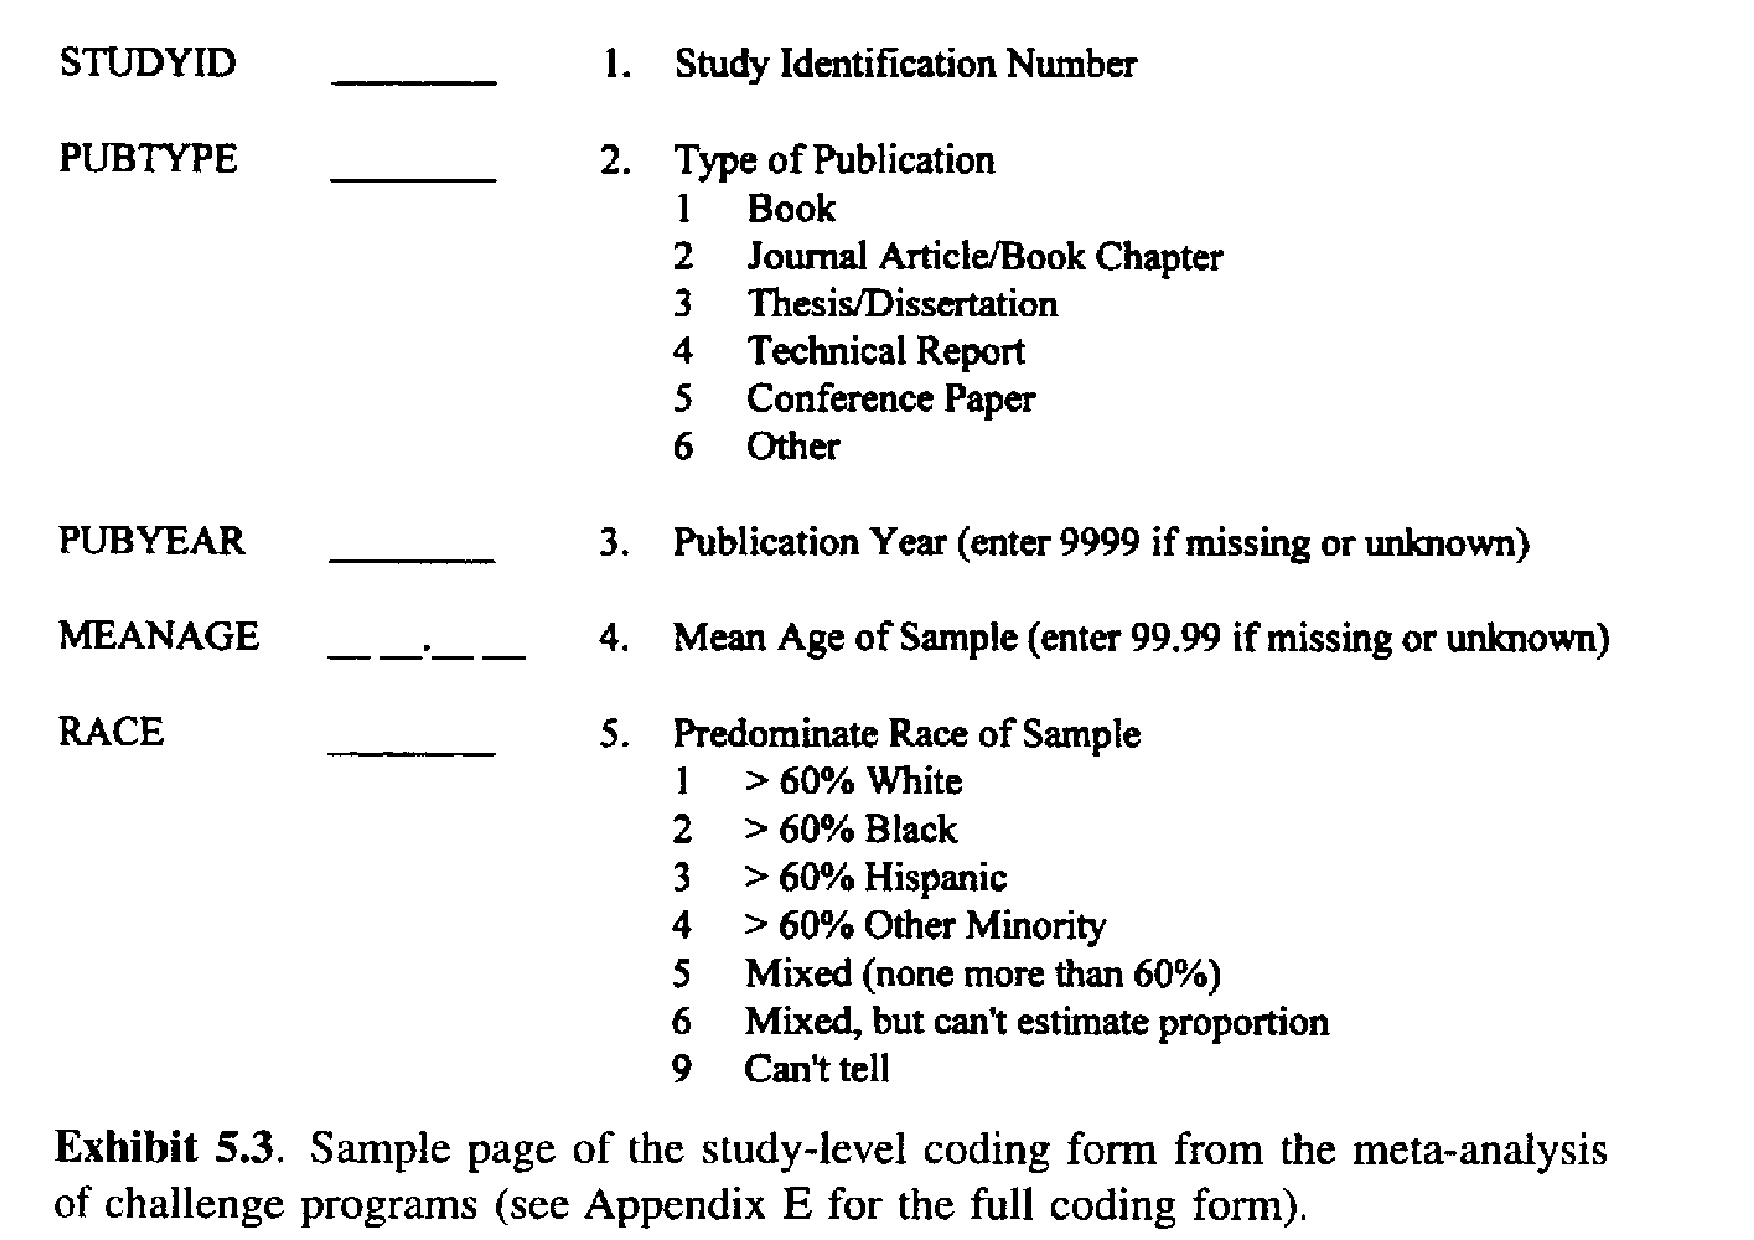
\includegraphics[scale = 0.3]{figKodierschema.pdf}
\end{frame}


\begin{frame}
  \frametitle{Was ist ein (empirischer) Forschungsbefund?}
  %%
  \begin{small}
    \begin{itemize}[<+->]
    \item Glass (1976: 6) weist die \emph{Effektstärke} als Mittelwertsdifferenz zwischen Experimental- und
      Kontrollgruppe aus, die durch Division mit der Gruppenvarianz (angenommen wird eine Gleichheit der
      Gruppenvarianzen) standardisiert wird.
    \item Nach Rosenthal (1991) beschreibt ein Forschungsbefund den Zusammenhang zwischen Variable $X$ und Variable
      $Y$. Dieser Zusammenhang enthält zwei Elemente:
      \begin{enumerate}
      \item ein Schätzer der Größe des Zusammenhangs (Effektstärke, engl. "`effect size"').
      \item eine Maßzahl für die Reliabilität der Effektgröße (Standardfehler, Konfidenzintervalle, $p$-Wert).
      \end{enumerate}
    \item Allgemein lässt sich ein Forschungsbefund definieren als "`[\ldots] statistical representation of one
      empirical relationship involving the variable(s) of interest to the meta-analysis measured on a single subject
      sample."'(Lipsey/Wilson 2000: 35)
    \end{itemize}
  \end{small}
\end{frame}



\begin{frame}
  \frametitle{Effektstärke}
  %%
  \begin{itemize*}
  \item Die wesentliche Eigenschaft einer Effektstärke ist nach Hedges\,/\,Olkin (1985: 7) ihre Skaleninvarianz
    (ermöglicht die Vergleichbarkeit zwischen Studien).
  \item Wünschenswerte Eigenschaften von Effektstärken sind zudem Informationen über \emph{Größe} und \emph{Richtung}
    des Zusammenhangs zwischen Variablen.
  \end{itemize*}
\end{frame}

\begin{frame}
  \frametitle{Von der Hypothese zur Effektstärke}
  %%
  \begin{itemize}[<+->]
  \item Unterschieds- oder Zusammenhangshypothesen
    \begin{itemize}
    \item Unterschiedshypothese: "`Wenn Jugendliche eine Klasse wiederholen müssen, dann steigt ihr Schwänzrisiko."'
    \item Zusammenhangshypothese: "`Je schlechter das Klassenklima vom einzelnen Schülern bewertet wird, desto höher
      auch das individuelle Schwänzrisiko."'
    \end{itemize}
  \item Gerichtete oder ungerichtete Hypothesen
    \begin{itemize}
    \item Unterschiedshypothesen (Wenn\ldots dann) und Zusammenhangshypothesen sind \emph{gerichtete} Hypothesen.
    \item Ungerichtete Hypothesen behaupten lediglich einen Unterschied, ohne jedoch eine Richtung (besser --
      schlechter, höher -- niedriger etc.) vorzugeben.
    \end{itemize}
\end{itemize}
\end{frame}


\begin{frame}
  \frametitle{Typen von Effektstärken\,/\,Forschungsbefunden (1)}
  %
  \begin{itemize}[<+->]
  \item Kontinuierliche Merkmale:
    \begin{itemize}
    \item Maßzahlen der $r$-Familie: z.B. $r$, ($\phi$), $r_{pb}$ und $\rho$
    \item Maßzahlen der $d$-Familie: z.B. Hedges' $g$, Glass' $\Delta$ und Cohen's $d$
    \end{itemize}
  \item Dichotome (kategoriale) Merkmale: z.B. odds ratio, risk ratio, $\phi$
  \item Teststatistiken (etwa $t$-, $F$- oder $\chi^2$-Werte)
  \item Narrative Darstellung signifikant positiver, negativer oder nichtsignifikanter Effekte
  \item $p$-Werte (kond. Wahrscheinlichkeit der fälschlichen Zurückweisung der $H_0$, gegeben, dass in GG die $H_0$
    gilt; $\alpha$-Fehlerwahrscheinlichkeit)
  \item \ldots
  \end{itemize}

  (mehr Informationen zu ES auf den Folien \pageref{sec:effectstaerken}ff verfügbar)

\end{frame}



\begin{frame}
  \frametitle{Typen von Effektstärken\,/\,Forschungsbefunden (2)}
  %%
  Effektstärken (besser: Forschungsbefunde) lassen sich aber auch nach der Anzahl der Variablen unterscheiden:
    \begin{itemize}
    \item Univariate Effektstärken (bspw. Anteile, Mittelwerte)
    \item Bivariate Effektstärken (bspw. $d$, $r$, odds ratio)
    \item Multivariate Effektstärken (bspw. Regressionskoeffizienten)
    \end{itemize}
  \end{frame}



\begin{frame}
  \frametitle{Welche meta-analytischen Verfahren gibt es für die verschiedenen Formen von Forschungsbefunden?}
  \begin{enumerate}
  \item Vote counting
  \item Zusammenfassen von Signifikanzwerten
  \item Zusammenfassen von Effektstärken (Effektstärkensynthese)
  \item Zusammenfassen von Korrelationsmatrizen
  \item \ldots
  \end{enumerate}
\end{frame}


\begin{frame}
  \frametitle{Ein Vorgriff auf das Berechnen einer mittleren Effektstärke}
  \begin{itemize}[<+->]
  \item Auf Grundlage der Ergebnisse ($T_j$) von $k$ unabhängigen Studien wird
    im einfachsten Fall eine mittlere Effektstärke ($\overline{T}$) als
    gewichtetes arithmetisches Mittel berechnet:
    \begin{equation*}
      \overline{T} = \frac{\sum\limits^k_{j=1}{w_j \times T_j}}{\sum\limits^k_{j=1}{w_j}}
    \end{equation*}

  \item Neben den ES werden auch noch \alert<+->{Gewichte} benötigt:
    \begin{itemize}
    \item Fallzahl ($w_j = n_j$)
    \item Inverse quadrierte Standardfehler (Fehlervarianz): $w_j = \frac{1}{SE_j^2}$
    \end{itemize}
  \end{itemize}
\end{frame}


\begin{frame}[plain]
  \frametitle{Abhängige Effektstärken}\label{slide:abhaeng-es}
  
  \begin{footnotesize}
    Wie entstehen abhängige Effektstärken?
    \begin{itemize}
    \item Multiple Befundstatistiken pro Person (bspw. mehrere Testergebnisse; hierarchische Regressionsmodelle).
    \item Verschiedene Treatment-Gruppen haben eine gemeinsame Kontrollgruppe.
    \item \ldots
    \end{itemize}

    Umgang mit abhängigen ES:
    \begin{itemize}
    \item Die "`beste"' (oder "`mittlere"') ES wählen.
    \item Zunächst pro Set abh. ES eine Meta-Analyse durchführen (Stufe 1) und
      dann eine zweite Meta-Analyse über die gemittelten ES durchführen (Stufe
      2).
    \item Bei multiplen ES (mehrere abh. Variablen) pro Personen pro Gruppe eine
      Meta-Analyse durchführen.
    \item Multivariate Meta-Analyse (Korrelationsmatrix muss vorliegen)
    \item Mehrebenen-Meta-Analyse
    \end{itemize}

    \citep[Quellen: ][]{kim_degree_2010, lambert_meta-analysis_1996,
      raudenbush_modeling_1988, thompson_impact_2013}
  \end{footnotesize}
\end{frame}



\section{Effektstärken (ES)}\label{sec:effectstaerken}

\begin{frame}\frametitle{Effektstärkenschätzer und -parameter}

  Bezüglich des Umgangs mit Effektstärken im Rahmen einer Meta-Analyse ist die
  folgende Unterscheidung wichtig:
  \begin{itemize}
  \item (Effektstärken-)\emph{Schätzer} werden in den Publikationen berichtet
    und basieren auf einer \emph{bestimmten} Stichprobe (\emph{sample effect
      sizes}).
  \item (Effektstärken-)\emph{Parameter} repräsentieren den \emph{wahren} Wert
    in der Grundgesamtheit (\emph{population (or true) effect size}).
  \end{itemize}

  Ein Ziel von Meta-Analyse ist, mit Hilfe der Effektstärken\emph{schätzer}
  den Populationsparameter zu schätzen. Neben dem eigentlichen ES-Schätzer wird
  (fast) immer auch der \emph{Standardfehler} als Gewicht benötigt.
   (Campbell Collaboration 2009: 5).
\end{frame}


\begin{frame}\frametitle{Übersicht und weiterführende Informationen}
  \begin{itemize}
  \item Hier werden
    \begin{itemize}
    \item die Produkt-Moment-Korrelation $r$,
    \item Cohens $d$,
    \item Hedges $g$,
    \item das Odds Ratio sowie
    \item der semi-partielle Korrelationskoeffizient (für Koeffizienten von
      multiplen linearen Regressionsmodellen) näher erläutert.
    \end{itemize}
  \item Gute Übersichten liefern u.a.
    \begin{itemize}
    \item \citet{borenstein_introduction_2009}, \citet{lipsey_practical_2001}
    \end{itemize}
  \end{itemize}
\end{frame}


\subsection{Effektstärken der $r$-Familie}


\begin{frame}
  \frametitle{Übersicht}
  %%
  \begin{itemize}[<+->]
  \item Produkt-Moment-Korrelation $r$ von (Bravais und) Pearson (beide Merkmale haben metrisches Skalenniveau)
  \item Korrelationskoeffizient nach Spearman (beide Merkmale haben ordinales Skalenniveau)
  \item Punkt-biserale Korrelation (ein Merkmal dichotom, ein Merkmal metrisch)
  \item \ldots
  \end{itemize}
  (Borenstein et al. 2009: 23ff)
\end{frame}


\begin{frame}[shrink = 5]
  \frametitle{Produkt-Moment-Korrelation}
  \framesubtitle{Eigenschaften der Effektstärke}
  %%
  \begin{itemize}[<+->]
  \item Pearsons $r$ errechnet sich aus der normierten Kovarianz und misst die Stärke des Zusammenhanges zweier Variablen.
  \item Der Korrelationskoeffizient liegt zwischen $-1$ (bei vollständig gegenläufigem Zusammenhang) und $+1$ (bei
    vollständig gleichläufigem Zusammenhang).
  \item Pearsons r ist ebenso wie die Kovarianz bei fehlendem Zusammenhang gleich 0.
  \item Der Korrelationskoeffizient kann nur für metrische Daten angewandt werden. Eine Ausnahme sind zwei dichotome
    Variablen, die 0/1 kodiert sind. In diesem Fall entspricht der Korrelationskoeffizient der Chi-Quadrat-basierten Maßzahl $\phi$.
  \end{itemize}
\end{frame}


\begin{frame}
  \frametitle{\large{Der Korrelationskoeffizient r von Bravais und Pearson}}
  \framesubtitle{Definition der Effektstärke}
  %%
  Pearsons $r$ lässt sich auch als die Kovarianz von $X$ und $Y$ ($S_{XY}$) dividiert durch das
  Produkt der Standardabweichungen von $X$ und $Y$ ($S_X$ und $S_Y$) definieren.
  % Durch die Normierung der Kovarianz fallen zum einen die Dimensionen der Ausgangsvariablen weg, zum anderen liegt der
  % Wertebereich des Koeffizienten immer zwischen $-1$ und +1. So können auch die unterschiedlichsten Verteilungen
  % miteinander verglichen werden.
  \begin{equation}
    r = \frac{S_{XY}}{S_X \cdot S_Y}
  \end{equation}
  mit:\\
  \begin{equation}
    S_{XY} = \frac{1}{n-1}\sum\limits^n_{i = 1}(x_i - \overline{x}) \cdot (y_i - \overline{y})
  \end{equation}

  \begin{equation}
    S_x = \sqrt{\frac{1}{n-1} \sum\limits^n_{i = 1} (x_i - \overline{x})^2} \text{  und  }
    S_y = \sqrt{\frac{1}{n-1} \sum\limits^n_{i = 1} (y_i - \overline{y})^2}
  \end{equation}
\end{frame}


\begin{frame}\frametitle{Die Fisher Z-Transformation}
  %%
  Bei der Befundsynthese von Korrelationskoeffizienten gilt es zu beachten, dass diese (i.A.) erst transformiert werden
  müssen. Diese Transformation hat zwei Gründe:
  \begin{enumerate}[<+->]
  \item Der Korrelationskoeffizient ist nicht normalverteilt.
  \item Der Standardfehler lässt sich nur für den transformierten Korrelationskoeffizienten bestimmen, da die
    Z-Transformation varianzstabilisierend ist und die Varianz von $z_r$ nicht von $r$ abhängt.
  \end{enumerate}
  \pause
  Es gilt dann:
  \begin{itemize}[<+->]
  \item Z-Transformation von $r$: $z_r=0.5 \cdot ln(\frac{1+r}{1-r})$.
  \item Standardfehler für $z_r$: $SE_{z_r}=\frac{1}{\sqrt{N-3}}$ mit $N$: Fallzahl.
  \item Rücktransformation $z_r$ zu $r$: $r=\frac{e^{2 \cdot z_r}-1}{e^{2 \cdot z_r}+1}$.
  \end{itemize}
\end{frame}


\begin{frame}\frametitle{Beispiel Fisher Z-Transformation}
  
  \begin{itemize}
  \item Gegeben sind: $r=0.13$ und $n=123$
  \item Fisher Z-transformierte Korrelation: $z_r = 0.5 \cdot
    \ln(\frac{1+0.13}{1-0.13})$ = 0.1307
  \item Standardfehler:
    $SE_{z_r}=\frac{1}{\sqrt{123-3}}$=0.0913
  \item Rücktransformation: $r=\frac{e^{2 \cdot 0.1307} -1}{e^{2 \cdot 0.1307} +
      1}$ = 0.13
  \end{itemize}
  
\end{frame}


\subsection{Effektstärken der $d$-Familie}

\begin{frame}
  \frametitle{Übersicht}
  %%
  \begin{itemize}[<+->]
  \item Die abhängige Variable ist metrisch skaliert, die unabhängige Variable
    ist ein (dichotomer) Faktor (Gruppenmerkmal, Pre-Post-Vergleich).
  \item Unstandardisierte Mittelwertdifferenz
    \begin{itemize}
    \item Für zwei unabhängige Gruppen
    \item Für abhängige Gruppen (etwa Pre-Post-Tests) (wird nicht weiter erläutert)
    \end{itemize}
  \item Standardisierte Mittelwertdifferenzen (Cohens $d$, Hedges $g$)
    \begin{itemize}
    \item Für zwei unabhängige Gruppen
    \item Für abhängige Gruppen (etwa Pre-Post-Tests) (wird nicht weiter erläutert)
    \end{itemize}
  \item \ldots
  \end{itemize}
  (Borenstein et al. 2009: 22ff)
\end{frame}


\begin{frame}\frametitle{Unstandardisierte Mittelwertdifferenz}

  Die unstandardisierte Mittelwertdifferenz zweier unabhängiger Mittelwerte
  $\mu_1$ und $\mu_2$ ist definiert als:

  \begin{equation}
    \Delta = \mu_1 - \mu_2,
  \end{equation}

  Die Schätzung von $\widehat{\Delta} = D$ erfolgt über zwei unabhängige
  Stichprobenmittelwerte $\overline{Y_1}$ und $\overline{Y_1}$:

  \begin{equation}
    D = \overline{Y_1} - \overline{Y_1}.
  \end{equation}
  
\end{frame}



\begin{frame}[plain, shrink]\frametitle{Varianz der unstandardisierten
    Mittelwertdifferenz}\label{sec:effektstarken-der-d}

  \begin{itemize}
  \item Seien $S_1$ und $S_2$ die beiden Standardabweichungen von $Y_1$ und
    $Y_2$ und angenommen, diese unterscheiden sich \emph{nicht} in der
    Population, dann ergibt sich die Varianz von $D$ als:
    
    \begin{equation}
      V_D = \frac{n_1 + n_2}{n_1n_2}S^2_{pooled} 
    \end{equation}
    
    mit
    
    \begin{equation}\label{eq:sd_pooled}
      S_{pooled} = \sqrt{\frac{(n_1-1)S^2_1 + (n_2-1)S^2_2}{n_1+n_2-2}}.
    \end{equation}
    
  \item Für unterschiedliche Populationsstandardabweichungen ergibt sich die Varianz
    von $D$ nach:
    
    \begin{equation}
      V_D = \frac{S^2_1}{n_1} + \frac{S^2_2}{n_2}.
    \end{equation}
  \end{itemize}
  
  Der Standardfehler von $D$ ergibt sich aber immer nach: 

  \begin{equation}
    SE_D = \sqrt{V_D}.
  \end{equation}
\end{frame}


\begin{frame}\frametitle{Beispiel unstandardisierte Mittelwertdifferenz}
  \begin{itemize}
  \item Gegeben sind:
    \begin{itemize}
    \item $\overline{Y}_1=103$, $S_1=5.5$, $n_1=50$
    \item $\overline{Y}_2=100$, $S_2=4.5$, $n_2=50$.
  \end{itemize}
  \item $D$ ist: $103-100=3$
  \item $SE_D$ ist (angenommen $\sigma_1 = \sigma_2$):
    \begin{itemize}
    \item $S_{pooled}=\sqrt{\frac{(50-1)5.5^2 + (50-1)4.5^2}{50+50-2}}=5.0249$
    \item $V_D = \frac{50+50}{50 \cdot 50} \cdot 5.0249 = 1.0100$
    \item $SE_D= \sqrt{1.0100} = 1.0050$
  \end{itemize}
  \end{itemize}
  \vfill
  \citep[22]{borenstein_introduction_2009}
\end{frame}



\begin{frame}\frametitle{Standardisierte Mittelwertdifferenz (Cohens $d$)}

  Die standardisierte Mittelwertdifferenz zweier unabhängiger Mittelwerte
  $\mu_1$ und $\mu_2$ ist definiert als:

   \begin{equation}
     \delta = \frac{\mu_1 - \mu_2}{\sigma}, \text{ wobei } \sigma_1 = \sigma_2 =\sigma,
   \end{equation}
   Die Schätzung von $\widehat{\delta} = d$ erfolgt über die zwei
   Stichprobenmittelwerte $\overline{Y_1}$ und $\overline{Y_1}$:
   \begin{equation}
     d = \frac{\overline{Y_1} - \overline{Y_1}}{S_{within}} \text{ (für $S_{within}$ siehe Gleichung \ref{eq:sd_pooled})}.
   \end{equation}
 
 \end{frame}

 
 \begin{frame}\frametitle{Varianz der standardisierten
     Mittelwertdifferenz}

   Seien $S_1$ und $S_2$ die beiden Standardabweichungen von $Y_1$ und $Y_2$ und
   angenommen, diese unterscheiden sich \emph{nicht} in der Population, dann
   ergibt sich die Varianz von $d$ (approximiert) als:
    
   \begin{equation}
      V_d = \frac{n_1 + n_2}{n_1n_2}+ \frac{d^2}{2(n_1+n_2)} 
    \end{equation}
    
    und einem Standardfehler $SE_d$ von
    
    \begin{equation}
      SE_d=\sqrt{V_d}.
    \end{equation}
    
\end{frame}



 \begin{frame}\frametitle{Standardisierte Mittelwertdifferenz (Hedges $g$)}

   In kleinen Stichproben überschätzt $d$ die wahre Mittelwertsdifferenz
   $\delta$. Dies lässt sich durch eine von Hedges vorgeschlagene Korrektur
   beheben:
   
   \begin{equation}
     g = J \times d, \text{ wobei } J = 1-\frac{3}{4df - 1}.
   \end{equation}
   
   mit $df=n_1 + n_2 - 2$ (für unabhängige Gruppen). 
   
   Für die Varianz von $g$ gilt:
   
   \begin{equation}
     V_g=J^2 \cdot V_d
   \end{equation}
   
   und entsprechend gilt für den Standardfehler von $g$:
   
   \begin{equation}
     SE_g=\sqrt{V_g}.
   \end{equation}
 \end{frame}
 
 
\begin{frame}\frametitle{Beispiel standardisierte Mittelwertdifferenz}
  \begin{itemize}
  \item Gegeben sind:
    \begin{itemize}
    \item $\overline{Y}_1=103$, $S_1=5.5$, $n_1=50$
    \item $\overline{Y}_2=100$, $S_2=4.5$, $n_2=50$.
    \end{itemize}
  \item $d$ ist: $\frac{103-100}{5.0249}=0.5970$
  \item $SE_D$ ist (angenommen $\sigma_1 = \sigma_2$):
    \begin{itemize}
    \item $S_{pooled}=\sqrt{\frac{(50-1)5.5^2 + (50-1)4.5^2}{50+50-2}}=5.0249$
    \item $V_D = \frac{50+50}{50 \cdot 50} + \frac{0.5970^2}{2(50+50)} = 0.0418$
    \item $SE_D= \sqrt{0.0418} = 0.2044$
    \end{itemize}
  \item Hedges $g$ ist:
    \begin{itemize}
    \item Korrekturfaktor: $J=\left(1-\frac{3}{4 \cdot 98 - 1}\right)=0.9923$
    \item $g=0.9923 \cdot 0.5970 = 0.5924$
    \item $V_g = 0.9923^2 \cdot 0.0418=0.0411$
    \item $SE_g= \sqrt{0.0411}= 0.2028$
    \end{itemize}
  \end{itemize}
  \vfill
  \citep[26ff]{borenstein_introduction_2009}
\end{frame}


\subsection{Kategoriale Effektstärken}

\begin{frame}\frametitle{Übersicht}
 
  Unter kategorialen Effektstärken werden vor allem Assoziationsmaße verstanden, die auf $2 \times 2$-Tabellen basieren:
  \begin{itemize}
  \item Risiko-Verhältnis (\emph{risk ratio})
  \item Chancenverhältnis (\emph{odds ratio})
  \item Risiko-Differenz (\emph{risk difference})
  \item Phi-Koeffizient
  \item \ldots
  \end{itemize}
\end{frame}


\begin{frame}\frametitle{Das Odds Ratio (1)}
  \begin{itemize}
  \item Eine \emph{Chance} (\emph{odds}) ist definiert als die
    Wahrscheinlichkeit $p(A)$, dass ein Ereignis A eintritt, geteilt durch die
    Gegenwahrscheinlichkeit $1-p(A)$, also:
    \begin{equation}
      Odds = \frac{p(E)}{1-p(E)}
    \end{equation}
  \item Das Chancenverhältnis (Odds Ratio) vergleicht nun die Chancen für Ereignis A über
    zwei Gruppen (z.B. Männer/Frauen, Control/Treatment ). Angenommen,
    \begin{itemize}
    \item in der Kontrollgruppe sterben 10,
    \item in der Treatment-Gruppe aber nur 5 von 100 Patienten. Daraus resultiert folgende Tabelle:
      \begin{tabular}{|r|c|c|}
        \hline
        & Control (0) & Treatment (1) \\
        \hline
        Alive (0) & 90    & 95    \\
        Death (1) & 10    & 5     \\
        \hline
      \end{tabular}
      \end{itemize}   
  \end{itemize}
\end{frame}


\begin{frame}\frametitle{Das Odds Ratio (2)}
  \begin{itemize}
  \item Für die Kontrollgruppe gilt: $Odds_C = \frac{10/100}{1 - (10/100)} = \frac{1/10}{9/10} = \frac{10}{90} = \frac{1}{9} \approx 0.1111$
  \item Für die Treatment-Gruppe gilt: $Odds_T = \frac{5}{95} \approx 0.0526$
  \item Das Odds Ratio beträgt dann: $\frac{5/95}{1/9}=\frac{45}{95} = \frac{9}{19} \approx 0.4737$
  \end{itemize}

  Die Interpretation des Odds Ratio ist wie folgt:
  \begin{itemize}
  \item Das Odds ratio kann Werte von 0 bis $+\infty$ annehmen und ist damit asymmetrisch verteilt.
  \item Ein Wert von 1 zeigt die statistische Unabhängigkeit der Merkmale an.
  \item Ein Wert kleiner 1 bzw. $[0;1)$ zeigt einen negativen Zusammenhang an.
  \item Ein Wert größer 1 bzw. $(1; \infty)$ zeigt einen positiven Zusammenhang an.
  \end{itemize}
\end{frame}
    


\begin{frame}\frametitle{Das Odds Ratio (3)}

Gilt allgemein die folgenden Tabellennotation  

\begin{center}
  \begin{tabular}{|r|c|c|}
    \hline
    & Control (0) & Treatment (1) \\
    \hline
    Alive (0) & A  & B   \\
    Death (1) & C  & D   \\
    \hline
  \end{tabular}
\end{center}

dann lässt sich das Odds Ratio ($\alpha$) schneller nach folgender Formel berechnen:

\begin{equation}
  \alpha = \frac{AD}{BC}
\end{equation}
\end{frame}
    

\begin{frame}\frametitle{Das Odds Ratio (4)}

  \begin{itemize}
  \item Ähnlich wie bei der PM-Korrelation, so muss auch das Odds Ratio in einer
    Meta-Analyse zunächst tranformiert (logarithmiert) werden (nicht normalverteilt,
    Standardfehler nicht bestimmt für Originalskala), also $ln(Odds Ratio) = ln(\alpha)$ (natürlicher Logarithmus).
  \item Die Rücktransformation erfolgt über die Exponentialfunktion: $exp(ln(\alpha))$.
  \item Die (approximierte) Varianz für $ln(\alpha)$ ist: 
    \begin{equation}
      V_{ln(\alpha)}= \frac{1}{A} + \frac{1}{B} + \frac{1}{C} + \frac{1}{D}
    \end{equation}
  \item Der (appr.) Standardfehler ist: $SE_{ln(\alpha)} = \sqrt{V_{ln(\alpha)}}$
  \end{itemize}
\end{frame}


\begin{frame}\frametitle{Beispiel Odds Ratio}
  \begin{itemize}
  \item Gegeben ist die folgende Tabelle:
    \begin{center}
      \begin{tabular}{|r|c|c|}
        \hline
        & Control (0) & Treatment (1) \\
        \hline
        Alive (0) & 90    & 95    \\
        Death (1) & 10    & 5     \\
        \hline
      \end{tabular}
    \end{center}
  \item Das Odds Ratio ist: $\alpha = \frac{90 \cdot 5}{10 \cdot 95} \approx 0.4737$
  \item Die Varianz beträgt: $V_{ln(\alpha)}= \frac{1}{90} + \frac{1}{95} + \frac{1}{10} + \frac{1}{5} \approx 0.3216$
  \item Der Standardfehler: $SE_{ln(\alpha)} = \sqrt{0.3216} = 0.5671$
  \end{itemize}
\end{frame}



\subsection{Regressionskoeffizienten}

\begin{frame}\frametitle{Überblick}

  \begin{itemize}
  \item Die Synthese von Regressionskoeffizienten in Meta-Analysen ist schwierig \citep[333ff.]{aloe_advances_2011}: 
    \begin{itemize}
    \item Regressionskoeffizienten (RK) für den \emph{focal predictor} von Modellen mit unterschiedlichen abhängigen
      Variablen (damit auch unterschiedliche Schätzverfahren) können i.d.R. nicht zusammengefasst werden.
    \item Der Wert eines RK hängt u.a. von der Existenz anderer Prädiktoren
      sowie dem Ausmaß der Interkorrelation aller Prädiktoren ab (Kollinearität).
    \item Unterschiedliche Operationalisierungen (Skalen) von abhängiger und unabhängiger (\emph{focal predictor}) Variable.    \end{itemize}
  \item Bislang existieren vor allem Verfahren für das \emph{allgemeine lineare Modell} ("`lineare Regression"').
  \end{itemize}   
\end{frame}



\begin{frame}
  \frametitle{Ansätze zur Synthese linearer Regressionsmodelle}
  
  \begin{itemize}
  \item Synthese unstandardiserter Koeffizienten mit Hilfe eines GLS-Ansatzes
    (benötigt aber die Varianz-Kovarianzmatrix des Regressionsmodells)
    \citep{becker_synthesis_2007}
  \item Standardisierte Regressionskoeffizienten \citep{kim_standardized_2011}
  \item "`Partial effect sizes"' (nur dichotome Prediktoren) \citep{keef_meta-analysis_2004}
  \item t-Statistiken \citep{stanley_metaregression_1989}
  \item Der semi-partielle Korrelationskoeffizient ($r_{sp}$; \emph{semi-partial correlation}) \citep{aloe_effect_2011, aloe_advances_2011}
  \item \ldots
  \end{itemize}
\end{frame}


\begin{frame}[plain ]
  \frametitle{Der semi-partielle Korrelationskoeffizient}
  
  \begin{equation}
    r_{sp} = sgn(t_f)\sqrt{r^2_Y - r^2_{Y(f)}}
  \end{equation}
  
  mit:\\
  $sgn$: Vorzeichenfunktion, gibt das Vorzeichen der t-Statistik zurück\\
  $t_f$: t-Statistik für Regressionskoeffizient des \emph{focal predictor}\\
  $r^2_Y$: Erklärte Varianz Gesamtmodell \\
  $r^2_{Y(f)}$: Erklärte Varianz für das Modell ohne \emph{focal predictor}
  
  \vspace{2ex}
  Besser geeignet ist aber die nachfolgende Formel:
  
  \begin{equation}
    r_{sp} = \frac{t_f \sqrt{(1-r^2_Y)}}{\sqrt{(n-p-1)}}
  \end{equation}
  
  mit:\\
  $n$: Fallzahl des Regressionsmodells\\
  $p$: Gesamtanzahl unabhängiger Variablen
     
\end{frame}



\begin{frame}
  \frametitle{Gemeinsame Meta-Analysen von $r_{sp}$ und $r$ möglich?}
  
  \begin{itemize}
  \item $r_{sp}$ sind gewöhnlich kleiner als PM-Korrelationen ($r$).
  \item Beide können gemeinsam in einer Meta-Analyse verwendet werden, aber im
    Rahmen einer Meta-Regression gilt es zu prüfen, ob sich beide Korrelationstypen
    systematisch unterscheiden \citep[346]{aloe_advances_2011}.
  \item Für eine Beispielanwendung siehe \citet{aloe_teacher_2009}.
  \end{itemize}
\end{frame}



\begin{frame}
  \frametitle{Varianz des semi-partiellen Korrelationskoeffizienten}
  Die Varianz für $r_{sp}$ lässt sich wie folgt schätzen:
  
  \begin{equation}
    V_{r_{sp}}= \frac{r^4_Y-2r^2_Y+r^2_{Y(f)}+1-r^4_{Y(f)}}{n}
  \end{equation}

  Unbekannt ist dabei meistens der Term $r^2_{Y(f)}$. Dieser ergibt sich aber aus:
  
  \begin{equation}
    r^2_{Y(f)}=r^2_Y - r^2_{sp}
  \end{equation}
  
\end{frame}


\begin{frame}
  \frametitle{Beispiel semi-partieller Korrelationskoeffizient}\label{slide:chaney-tab}

  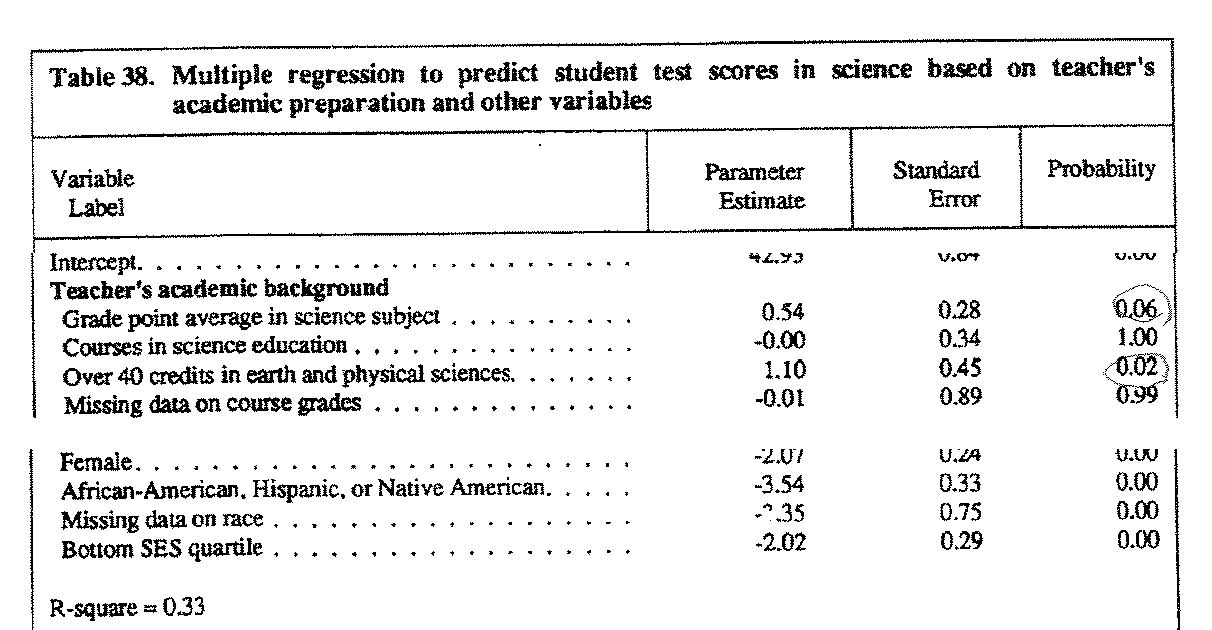
\includegraphics[width=0.9\linewidth]{f_chaney95_regtab.png}
    
  \citep[Quelle:][74; die Tabelle ist nicht vollständig dargestellt]{chaney_student_1995}
  
\end{frame}


\begin{frame}[plain]
  \frametitle{Beispiel semi-partieller Korrelationskoeffizient}
  
  Dem Tabellenausschnitt auf Folie \pageref{slide:chaney-tab} lassen sich
  folgende Informationen für den Effekt von "`Grade point average in science
  subject"' entnehmen:

  \begin{itemize}
  \item $t$-Statistik: 0.54/0.28=1.93
  \item $r_Y^2$ (R-square): 0.33
  \item N (nicht in Tabelle, siehe Fußnote)\footnote{Aloe \& Becker verwenden
      vermutlich die falsche Fallzahl (richtig: 24599), siehe
      \url{http://nces.ed.gov/pubs94/94378.pdf}, Fußnote 3}:
    26435
  \item p (Anzahl Prädiktoren): 26
  \end{itemize}
  
  Dann berechnet sich $r_{sp}$ nach (trotz kleinerer Fehler in Aloe \& Becker
  halte ich mich weitgehend an deren Darstellung):
  
  \begin{equation*}
    r_{sp}=\frac{1.9\sqrt{(1-0.33)}}{\sqrt{(26435-26-1)}}=0.0097
  \end{equation*}
    
  \citep[Quelle: ][346; kleine Typo in Beispielrechnung, $p=26$, nicht
  27]{aloe_advances_2011}
  
\end{frame}


\begin{frame}
  \frametitle{Beispiel Varianz des semi-partiellen Korrelationskoeffizienten}

  Zur Berechnung der Varianz von $r_{sp}$ fehlt noch $r^2_{Y(f)}$, d.h. die
  erklärte Gesamtvarianz für ein Modell \emph{ohne} den \emph{focal predictor}. 
  
  \begin{equation*}
    r^2_{Y(f)}=r^2_Y - r^2_{sp} = 0.33 - 0.0097^2 = 0.3299
  \end{equation*}
  
  Für die Varianz von $r_{sp}$ gilt dann:
  
  \begin{equation*}
    V_{r_{sp}} = \frac{0.1089 - 2 \cdot 0.33 + 0.3299 + 1 - 0.1088}{26435} = 
    0.000025 
  \end{equation*}
    
  Der Standardfehler beträgt:
  
  \begin{equation*}
    SE_{r_{sp}}=0.005
  \end{equation*}
  
  \citep[Quelle: ][347]{aloe_advances_2011}
  
\end{frame}



\subsection{Effektstärkenkonvertierung}

\begin{frame}
  \frametitle{Überblick}
  
  \begin{itemize}
  \item Unterschiedliche Studien berichten trotz gleicher/ähnlicher
    Fragestellung unterschiedliche Statistiken/Effektstärken.
  \item Viele bivariate Effektstärken lassen sich (approximativ) ineinander
    überführen.
  \item Anschließend lassen sich diese konvertierten Effektstärken gemeinsam im
    Rahmen einer Meta-Analyse analysieren.
  \item Hier wird nur eine kleine Auswahl gängiger Transformationsregeln
    vorgestellt. Weiterführende Darstellungen finden sich u.a. bei
    \begin{itemize}
    \item \citet{borenstein_introduction_2009},
    \item \citet{rosenthal_contrasts_2000},
    \item \citet{lipsey_practical_2001},
    \item \citet{higgins_cochrane_2008},
      \item \ldots
    \end{itemize}
  \item Die nachfolgenden Ausführungen basieren auf \citet[46ff.]{borenstein_introduction_2009}.
  \end{itemize}
\end{frame}


\begin{frame}
  \frametitle{Konvertierung zwischen $ln(\text{odds ratio})$ und $d$}

  \begin{equation}
    d = \ln(\text{odds ratio}) \cdot \frac{\sqrt{3}}{\pi}
  \end{equation}
  
  \begin{equation}
    V_d = V_{ln(\text{odds ratio})} \cdot \frac{3}{\pi^2}
  \end{equation}
  
  \begin{equation}
    \ln(\text{odds ratio})=d\frac{\pi}{\sqrt{3}}
  \end{equation}

    \begin{equation}
    V_{ln(\text{odds ratio})} = V_d \frac{\pi^2}{3}
  \end{equation}  

\citep[46ff]{borenstein_introduction_2009}
      
\end{frame}


\begin{frame}
  \frametitle{Konvertierung zwischen $r$ und $d$}

  \begin{equation}
    d = \frac{2r}{\sqrt{1-r^2}}
  \end{equation}
  
  \begin{equation}
    V_d = \frac{4V_r}{(1-r^2)^3}
  \end{equation}
  
  \begin{equation}
    r = \frac{d}{\sqrt{d^2+a}},
  \end{equation}
  
  wobei $a$ ein Korrekturfaktor für $n_1 \neq n_2$ ist:
  
  \begin{equation}
    a = \frac{(n_1+n_2)^2}{n_1n_2}
  \end{equation}
  
  \begin{equation}
    V_r = \frac{a^2V_d}{(d^2+a)^3}
  \end{equation}

  \citep[46ff]{borenstein_introduction_2009}
  
\end{frame}

  



%%% Local Variables:
%%% TeX-master: "ps2012gesis-ma-workshop.tex"
%%% End:
